    %!TEX encoding = UTF-8 Unicode 
\documentclass[usenames,dvipsnames]{beamer}

    \usetheme{metropolis}

   \usecolortheme{seahorse}
   
        \usepackage{pgfpages}
\usepackage{CJKutf8} 
\usepackage{tcolorbox}
\usepackage[textfont={small}]{caption}
\usepackage{dcolumn}


    \setbeamercovered{invisible}
    \usepackage{tikz}   
    \usetikzlibrary{shapes,arrows}
\usepackage{graphicx}% http://ctan.org/pkg/graphicx
\usepackage{booktabs}
    \usepackage{framed, color}
    \definecolor{shadecolor}{rgb}{1, 0.8, 0.3}
    % To remove the navigation symbols from
    % the bottom of slides%
 %\setbeameroption{show notes on second screen}
%\setbeameroption{show only notes}
    \setbeamertemplate{navigation symbols}{}
    %
  \setbeamercolor{section in head/foot}{fg=black, bg=structure.fg!20!white}

\usepackage[natbibapa]{apacite}
\bibliographystyle{apacite}
\bibpunct{(}{)}{;}{a}{}{,}

\usetikzlibrary{calc}


\tikzstyle{decision} = [diamond, draw, fill=blue!20, 
    text width=4.5em, text badly centered, node distance=3cm, inner sep=0pt]
\tikzstyle{block} = [rectangle, draw, fill=blue!20, 
    text width=6em, text centered, rounded corners, minimum height=4em]
\tikzstyle{line} = [draw, -latex']
\tikzstyle{cloud} = [draw, ellipse,fill=red!20, node distance=3cm,
    minimum height=2em]

\newcommand{\tikzmark}[1]{\tikz[overlay,remember picture] \node (#1) {};}
\newcommand{\DrawBox}[1][]{%
    \tikz[overlay,remember picture]{
    \draw[red,#1]
      ($(left)+(-0.2em,0.9em)$) rectangle
      ($(right)+(0.2em,-0.3em)$);}
}

\newenvironment{variableblock}[3]{%
  \setbeamercolor{block body}{#2}
  \setbeamercolor{block title}{#3}
  \begin{block}{#1}}{\end{block}}

\makeatletter
\setbeamertemplate{footline}
{
  \leavevmode%
  \hbox{%
  \begin{beamercolorbox}[wd=1\paperwidth,ht=2.25ex,dp=1ex,center]{author in head/foot}%
    \usebeamerfont{author in head/foot}%
    \insertsectionnavigationhorizontal{0.8\paperwidth }{}{}%
     \insertframenumber /  \inserttotalframenumber
 \end{beamercolorbox}}%
 % \begin{beamercolorbox}[wd=.3\paperwidth,ht=2.25ex,dp=1ex,right]{date in head/foot}%
   % \usebeamerfont{date in head/foot}\insertshortdate{}\hspace*{2em}
  \hspace*{2ex} 
  %\end{beamercolorbox}}%
  \vskip0pt%
}


\usepackage{graphicx}
\usepackage[caption=false]{subfig}
\usepackage{multicol}
\usepackage{color, colortbl}
\definecolor{Gray}{gray}{0.9}

%\definecolor{white}{white}{0.9}

%\setbeamercovered{white}
    %\usepackage{bm} % For typesetting bold math (not \mathbold)
    %\logo{\includegraphics[height=0.6cm]{yourlogo.eps}}
\title{Corruption information and vote share: \\ A meta-analysis and lessons for survey
experiments}
\author{Trevor Incerti}
\date{6 September 2019 \\


\vspace{0.5cm}
\scriptsize
Prepared for the Yale ISPS Experiments Workshop
}

\begin{document}
\maketitle

%%%%%%%%%%%%%%%%%%%%%%%%%%%%%%%%%%%

\section{Introduction}

\begin{frame}
\frametitle{Research Question}
\textbf{Do voters hold politicians accountable for corruption?}
\pause
\begin{itemize}
\item Key question of \textcolor{Cerulean}{electoral accountability}. 
\pause
\item ARPS review: ``Empirical evidence to date is \textcolor{Cerulean}{mixed}, and it often suggests that the electoral punishment of corruption is rather mild.'' \citep{de2017electoral} 
\pause
\item Recent explosion of experimental research on this subject. 
\pause
\item What have we learned from this research? Is evidence actually mixed?
\end{itemize}
\end{frame}

%%%%%%%%%%%%%%%%%%%%%%%%%%%%%%%%%%%

\section{Methods}

\begin{frame}[label = methods]
\frametitle{Meta-Analysis}
Meta-analysis of all \textcolor{Cerulean}{experimental} studies conducted to date. 
\pause
\begin{itemize}
\item \textcolor{Cerulean}{Treatment}: corruption information provision. 
\pause
\item \textcolor{Cerulean}{Outcome}: vote-share of corrupt politician.
\pause
\item Random assignment of corruption information $\rightarrow$ measurement of voting outcomes.
\pause
\item As treatments are not always assigned identically, I take steps to standardize where possible. \hyperlink{details}{\beamerbutton{Details}}
\pause
\item Includes both \textcolor{Cerulean}{published articles and working papers}.
\end{itemize}
\end{frame}

%%%%%%%%%%%%%%%%%%%%%%%%%%%%%%%%%%%

\begin{frame}[label = methods_2]
\frametitle{Meta-Analysis}
I use \textcolor{Cerulean}{fixed effects} and \textcolor{Cerulean}{random effects} estimation. 
\vspace{0.25cm}
\pause
\begin{itemize}
\item Random effects likely more appropriate in this case. 
\begin{itemize}
\item Fixed effects assumes one true effect size across all studies, with differences in effects due to sampling error.  \hyperlink{fixed_random}{\beamerbutton{Details}}
\item Random effects assumes effect sizes vary due to population heterogeneity, differences in treatment, etc.
\item In random effects, effect sizes are therefore assumed to represent a random sample of a distribution of effect sizes.
\end{itemize}
\vspace{0.25cm}
\item In this case, differences in estimated effect size between the two methods are minor. 
\end{itemize}
\end{frame}

%%%%%%%%%%%%%%%%%%%%%%%%%%%%%%%%%%%

\section{Results}

\begin{frame}
\frametitle{Results: Field Experiments}

\only<1>{
\begin{figure}
\hspace*{-11mm}
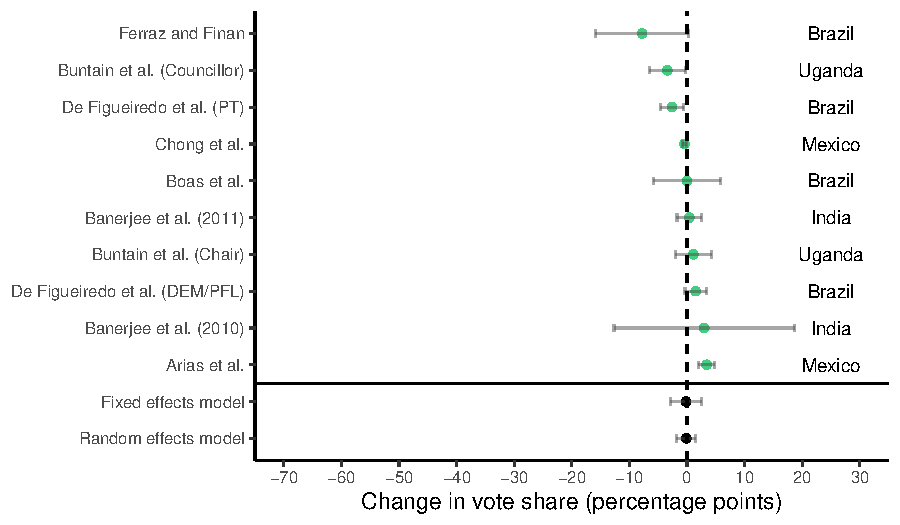
\includegraphics[scale=0.83]{../figs/field.pdf}
\end{figure}
}

\end{frame}

%%%%%%%%%%%%%%%%%%%%%%%%%%%%%%%%%%%

\begin{frame}
\frametitle{Results: Survey Experiments}

\only<1>{
\begin{figure}
\vspace*{-1cm}
\hspace*{-11mm}
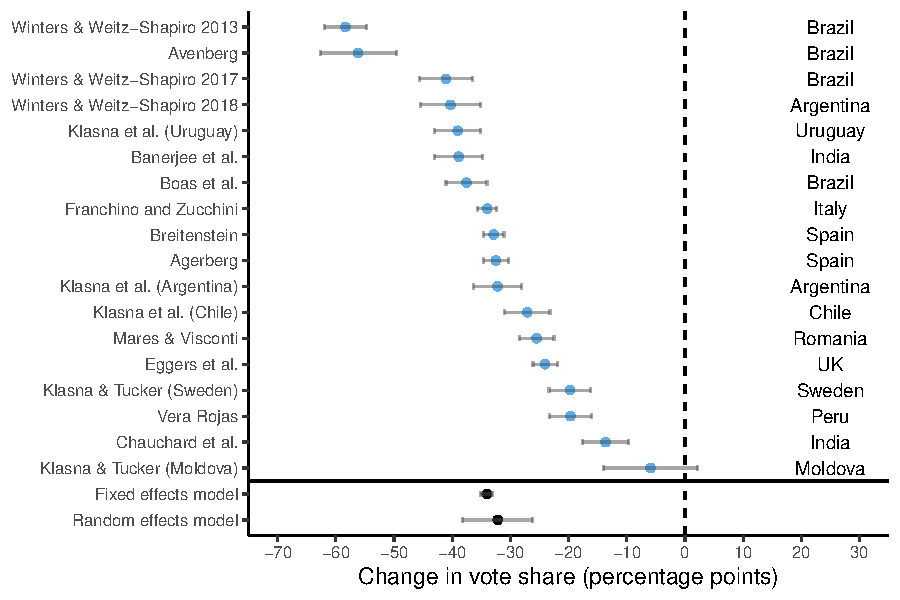
\includegraphics[scale=0.83]{../figs/survey.pdf}
\end{figure}
}

\end{frame}

%%%%%%%%%%%%%%%%%%%%%%%%%%%%%%%%%%%

\begin{frame}[label = results]
\frametitle{Results}
\begin{itemize}
\item Survey experiments estimate much larger negative treatment effects relative to field experiments. \hyperlink{lab}{\beamerbutton{Lab experiments similar to survey}}
\pause
\item Corrupt candidates punished by approximately \textcolor{Cerulean}{zero percentage points} in field experiments.
\pause
\item Punished by between \textcolor{Cerulean}{33 percentage points} (random effects) and \textcolor{Cerulean}{35 percentage points} (fixed effects) in survey experiments.
\vspace{0.05cm}
\end{itemize}
\end{frame}

%%%%%%%%%%%%%%%%%%%%%%%%%%%%%%%%%%%

\begin{frame}[label = heterogeneity]
\frametitle{Assessing within study heterogeneity}
How much heterogeneity across studies is accounted for by type of experiment?
\begin{itemize}
\item First estimate total amount of heterogeneity across all studies with random effects model.  
\pause
\item Next, estimate residual heterogeneity after including a categorical indicator for experiment type in the model. 
\pause
\begin{itemize}
\item Point estimate of this dummy (0 = field, 1 = survey) is equal to -0.33 (significant at 1\% level), the same as the overall estimate across all studies (with no moderator). \hyperlink{me_mod}{\beamerbutton{Results}}
\end{itemize}
\pause
\item Subtract residual heterogeneity from total heterogeneity and divide by total heterogeneity. 
\pause
\item 68\% of the total heterogeneity across studies accounted for by including a dummy variable for type of experiment.
\end{itemize}
\end{frame}

%%%%%%%%%%%%%%%%%%%%%%%%%%%%%%%%%%%
\section{Discussion}

\begin{frame}
\frametitle{Discussion}
What might account for the discrepancy between field and survey experiments?
\pause
\begin{itemize}
\item Publication bias and/or p-hacking
\pause
\item Social desirability bias
\pause
\item Survey context does not mirror real-world settings:
\begin{itemize}
\item Non-compliance
\item Differences in outcome choices
\item Costliness/decision complexity
\end{itemize}
\end{itemize}

\end{frame}

%%%%%%%%%%%%%%%%%%%%%%%%%%%%%%%%%%%

\begin{frame}[label=pub_bias]
\frametitle{Publication bias and p-hacking}
\textcolor{Cerulean}{No clear evidence of publication bias} within survey experiments:
\pause
\begin{itemize}
\item P-curve - virtually all results significant at 1\% level (not clustered around 0.05 or 0.01).
\item Tests for funnel plot asymmetry. \hyperlink{funnel}{\beamerbutton{Figures}}
\item P-value not a significant predictor of publication status. \hyperlink{p_ols_logit}{\beamerbutton{Table}}
\end{itemize}
\pause
Unclear with field experiments
\begin{itemize}
\item Five of eight papers published. Three unpublished papers all have null findings. \hyperlink{all_published}{\beamerbutton{Figure}}
\pause
\item Not enough data for formal tests. 
\end{itemize}

\end{frame}

%%%%%%%%%%%%%%%%%%%%%%%%%%%%%%%%%%%
\begin{frame}
\frametitle{Social desirability bias}
\begin{itemize}
\pause
\item Anti-corruption norms exist in most countries.
\pause
\item No costs to selecting the socially desirable option in hypothetical vignette. 
\pause
\item Voting against corruption in the abstract may therefore reflect the respondents’ actual preferences.
\pause
\item In actual election voters may discount information, or have strong material/ideological incentives to stick with candidate.
\end{itemize}

\end{frame}

%%%%%%%%%%%%%%%%%%%%%%%%%%%%%%%%%%%
\begin{frame}
\frametitle{Differences in experimental context: non compliance}

Treatments are weak and easily missed in field experiments. 
\begin{itemize}
\item In survey experiments ITT = ATE = CACE (LATE)
\item Field experiments measure ITT as they do not know the non compliance rate. Non compliance necessarily reduces the ITT.
\begin{itemize}
\item $ITT = CACE \times \pi_C$
\end{itemize}
\end{itemize}

\end{frame}

%%%%%%%%%%%%%%%%%%%%%%%%%%%%%%%%%%%
\begin{frame}
\frametitle{Differences in experimental context: outcome choice}
Choice set offered to voters is not necessarily identical across experiments. Example:

\begin{itemize}
\item Field experiment: Candidate A is randomly revealed to be corrupt, and voters can cast vote for corrupt candidate A, or candidate B, who may be clean or corrupt. 
\vspace{0.5cm}
\item Survey experiment: Candidate A is randomly revealed to be corrupt, and voters can cast vote for corrupt candidate A, or counterfactual Candidate A who \textit{is not} corrupt. 

\end{itemize}

\end{frame}

%%%%%%%%%%%%%%%%%%%%%%%%%%%%%%%%%%%
\begin{frame}
\frametitle{Differences in experimental context: complexity, costliness and conjoint experiments}
\textcolor{Cerulean}{Conjoint experiments}: Randomizing more candidate characteristics may capture variety of moderating factors and reduce social desirability bias.
\begin{itemize}
\pause
\item But, traditional method of analysis (comparing magnitudes of individual average marginal component effects) may be misleading. 
\end{itemize}

\end{frame}

%%%%%%%%%%%%%%%%%%%%%%%%%%%%%%%%%%%
\begin{frame}
\frametitle{Differences in experimental context: complexity, costliness and conjoint experiments}

\begin{figure}[!hb]
\hspace*{-11mm}
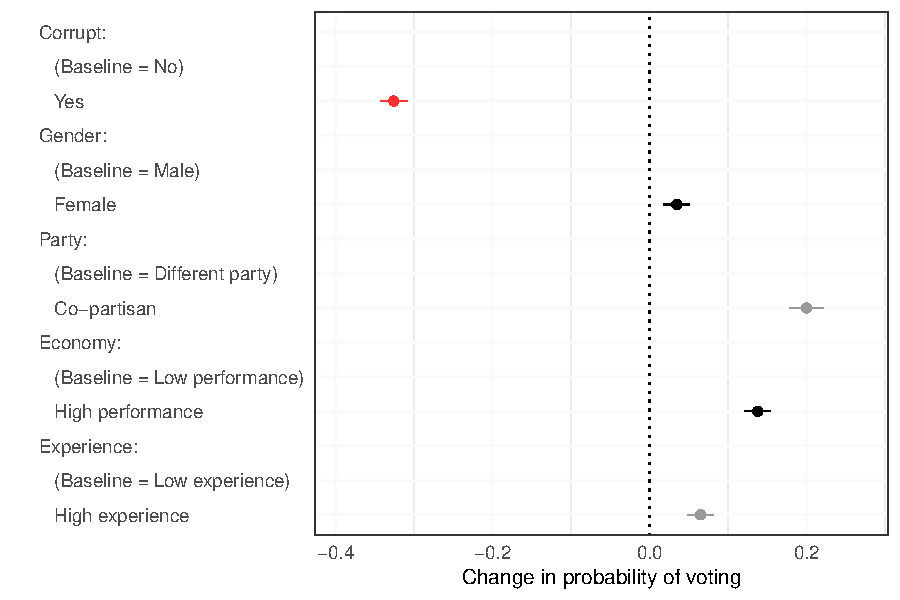
\includegraphics[scale = 0.7]{../figs/b_amce.pdf}
\caption{\citet{breitenstein2019choosing} conjoint: average marginal component effects}
\small
\vspace{-0.5cm}
\label{fig: b_amce}
\end{figure}

\end{frame}

%%%%%%%%%%%%%%%%%%%%%%%%%%%%%%%%%%%
\begin{frame}[label=conjoint]
\frametitle{Differences in experimental context: complexity, costliness and conjoint experiments}

\textcolor{Cerulean}{Proposal}: When researchers have strong theories about the \textcolor{Cerulean}{conditions that shape voter decision-making}, a more appropriate method may be to calculate average marginal effects in order to present predicted probabilities of voting for a candidate under these conditions.
\begin{itemize}
\item E.g. Compare the probability of voting for a \textcolor{Cerulean}{realistic candidate} with outlier characteristics such as corruption to the probability of voting for a realistic candidate without this characteristic. \hyperlink{b_conjoint}{\beamerbutton{Example 1}}  \hyperlink{fz_conjoint1}{\beamerbutton{Example 2}} \hyperlink{fz_conjoint1}{\beamerbutton{Example 3}}
\end{itemize}

\end{frame}


%%%%%%%%%%%%%%%%%%%%%%%%%%%%%%%%%%%
\begin{frame}[label=b_conjoint]
\frametitle{Differences in experimental context: complexity, costliness and conjoint experiments}

\begin{figure}[!hb]
\centering
\vspace*{-7mm}
\hspace*{-11mm}
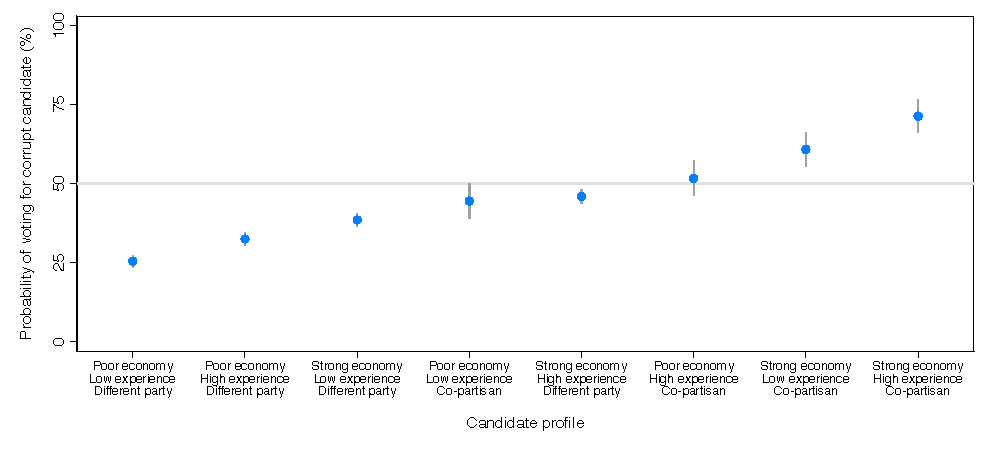
\includegraphics[scale = 0.77]{../figs/b_margins.pdf}
\caption{\citet{breitenstein2019choosing} conjoint: can the right candidate overcome corruption?}
\small
\label{fig: b_margins}
\end{figure}

\end{frame}

%%%%%%%%%%%%%%%%%%%%%%%%%%%%%%%%%%%
\begin{frame}
\frametitle{Differences in experimental context: complexity, costliness and conjoint experiments}

\small
\textcolor{Cerulean}{Proposal}: When we do not have strong theories about the conditions that shape voter decision-making, we can use regression trees to illuminate them. 

\begin{figure}[!hb]
\centering
\vspace*{-3mm}
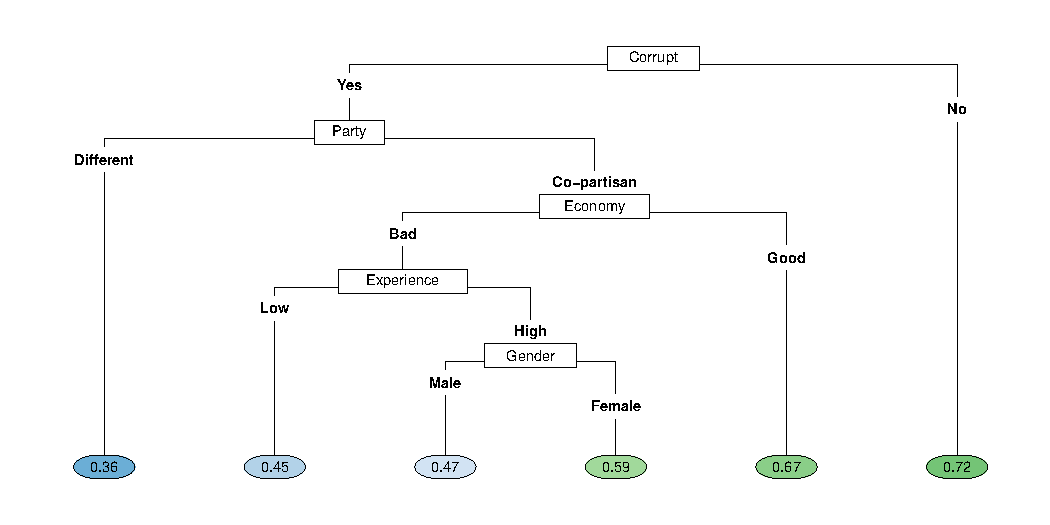
\includegraphics[scale = 0.54]{../figs/b_tree.pdf}
\vspace{-0.2cm}
\caption{\citet{breitenstein2019choosing} conjoint decision tree: predicted probabilities of voting for candidate}
\label{fig: b_tree}
\end{figure}


\end{frame}


%%%%%%%%%%%%%%%%%%%%%%%%%%%%%%%%%%%
\section{Conclusion}

\begin{frame}
\frametitle{Conclusion}
\begin{itemize}
\pause
\item Effect of corruption information on vote-choice \textcolor{Cerulean}{differs drastically} between field and survey experiments.
\begin{itemize}
\pause
\item \textcolor{Cerulean}{Zero} in field experiments.
\item \textcolor{Cerulean}{-33 to -35 percentage points} in survey experiments. 
\end{itemize}
\pause
\item Discrepancy does not seem to be driven by publication bias/p-hacking.
\pause
\item May arise from:
\begin{itemize} 
\pause
\item Social desirability bias
\pause
\item Survey context failing to mirror real-world settings:
\begin{itemize}
\item Non-compliance
\item Differences in outcome choices
\item Costliness/decision complexity
\end{itemize}
\end{itemize}
\end{itemize}
\end{frame}

%%%%%%%%%%%%%%%%%%%%%%%%%%%%%%%%%%%

\begin{frame}
\frametitle{Conclusion}
\begin{itemize}
\item Vote-choice \textcolor{Cerulean}{survey experiments} may provide information on the directionality of informational treatments in hypothetical scenarios, but point estimates they provide \textcolor{Cerulean}{may not be representative of real-world voting behavior}. 
\pause
\item Researchers should \textcolor{Cerulean}{exercise caution} when interpreting actions taken in hypothetical vignettes as indicative of real world behavior such as voting. 
\end{itemize}

\end{frame}

%%%%%%%%%%%%%%%%%%%%%%%%%%%%%%%%%%%

\begin{frame}
\frametitle{Feedback}
\begin{itemize}
\item Other possible reasons behind the discrepancy?
\pause
\vspace{0.25cm}
\item Are empirical tests of the reasons I have already identified necessary?
\pause
\vspace{0.25cm}
\item If so, what tests would you find convincing? 
\end{itemize}

\end{frame}

%%%%%%%%%%%%%%%%%%%%%%%%%%%%%%%%%%%
\appendix

\section{Supplemental material}

\begin{frame}[label=details, noframenumbering]
\frametitle{Analytical details \hyperlink{methods}{\beamerbutton{Back}}}
\begin{itemize}
\item Where there are multiple corruption treatments (e.g. varying source of information), I replicate the studies and code corruption as a binary treatment (0 = clean, 1 = corrupt).
\pause
\item Studies that use non-binary vote choices are rescaled into a binary vote choice.
\pause
\item Point estimates, standard errors and/or confidence intervals are not always explicitly reported (4 cases). In these cases standard errors are estimated by digitally measuring coefficient plots.
\pause
\item Two field experiments include general anti-corruption treatments not specific to candidates. Robustness check excludes these studies. 
\end{itemize}
\end{frame}

%%%%%%%%%%%%%%%%%%%%%%%%%%%%%%%%%%%

\begin{frame}[label=fixed_random, noframenumbering]
\frametitle{Fixed versus random effects estimation \hyperlink{methods_2}{\beamerbutton{Back}}}

Fixed effects: \\
\vspace{0.25cm}

$\hat{\theta} = \frac{\sum w_i \theta_i}{\sum w_i}$ where $w_i = \frac{1}{var_i}$ \\

\vspace{0.5cm}

Random effects: \\
\vspace{0.25cm}

$\hat{\theta} = u + u_i$ where $u_i \sim N(0, \tau^2)$ and: \\

\vspace{0.25cm}

$u$ is equal to the average ``true effect'', and $\tau^2$ is the heterogeneity amongst true effects. 

\end{frame}

%%%%%%%%%%%%%%%%%%%%%%%%%%%%%%%%%%%

\begin{frame}[label=lab, noframenumbering]
\frametitle{Lab experiments \hyperlink{results}{\beamerbutton{Back}}}

\begin{figure}[!htb]
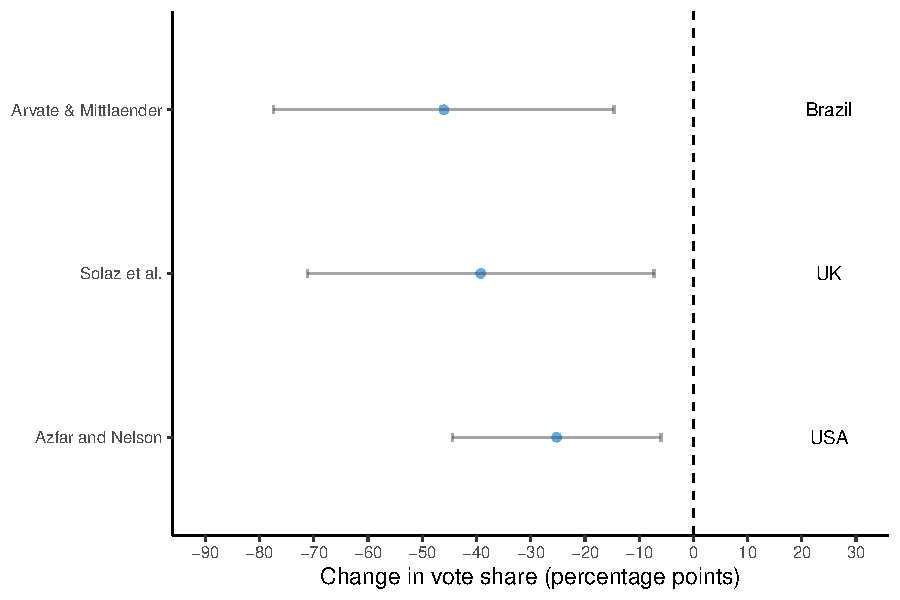
\includegraphics[scale=0.65]{../figs/lab.pdf}
\vspace{0.2cm}
\caption{Lab experiments: Average treatment effect of corruption information on vote share}.
\small
\vspace{-0.3cm}
\label{fig: lab}
\end{figure}
\end{frame}


%%%%%%%%%%%%%%%%%%%%%%%%%%%%%%%%%%%

\begin{frame}[label=supplemental, noframenumbering]
\frametitle{Robustness checks}

\begin{figure}[!hb]
\hspace*{-11mm}
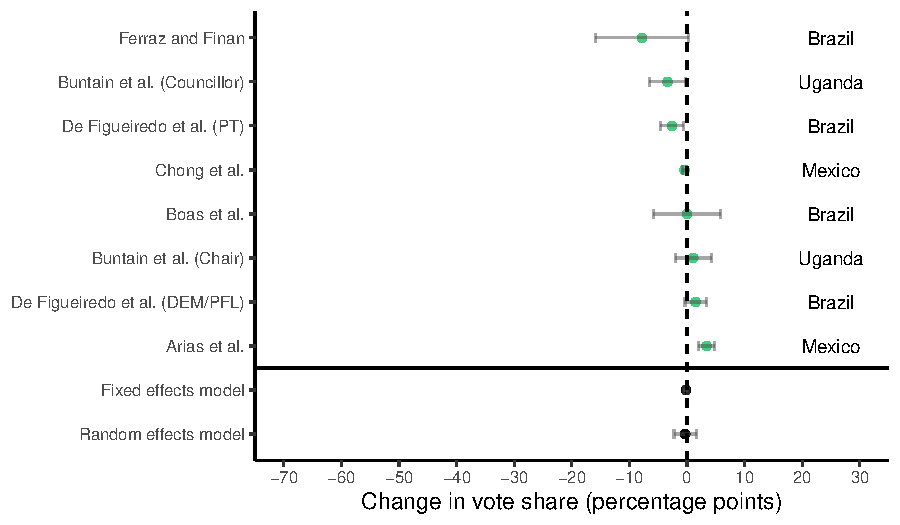
\includegraphics[scale = 0.75]{../figs/field_no_banerjee.pdf}
\vspace{-0.2cm}
\caption{Field experiments: Average treatment effect of corruption information on incumbent vote share (excluding \cite{banerjee2010can} and \citet{banerjee2011informed})}
\small
\vspace{-0.5cm}
\label{fig: field_no_banerjee}
\end{figure}
\end{frame}

%%%%%%%%%%%%%%%%%%%%%%%%%%%%%%%%%%%

\begin{frame}[label = me_mod, noframenumbering]
\frametitle{Mixed effects meta-analysis with survey experiment moderator \hyperlink{heterogeneity}{\beamerbutton{Back}}}


% Table created by stargazer v.5.2.2 by Marek Hlavac, Harvard University. E-mail: hlavac at fas.harvard.edu
% Date and time: Wed, Jan 29, 2020 - 17:55:53
\begin{table}[!htbp] \centering 
  \caption{Mixed effects meta-analysis with survey experiment moderator} 
  \label{me_mod} 
\begin{tabular}{@{\extracolsep{5pt}} ccc} 
\\[-1.8ex]\hline 
\hline \\[-1.8ex] 
Value & Estimate & 95\% CI \\ 
\hline \\[-1.8ex] 
Constant & -0.007 & -0.074 to 0.06 \\ 
 & (0.034) &  \\ 
Survey experiment moderator & -0.315 & -0.398 to -0.231 \\ 
 & (0.043) &  \\ 
Residual heterogenity with moderator & 0.011 & 0.005 to 0.017 \\ 
 & (0.003) &  \\ 
Heterogenity accounted for & 67.97\% &  \\ 
 &  &  \\ 
\hline \\[-1.8ex] 
\multicolumn{3}{l}{\parbox[t]{\textwidth}{\footnotesize \textit{Note:} Standard errors in parenthesis. Figures rounded to nearest thousandth decimal place.}} \\ 
\end{tabular} 
\end{table} 


\end{frame}

%%%%%%%%%%%%%%%%%%%%%%%%%%%%%%%%%%%

\begin{frame}[label=funnel, noframenumbering]
\frametitle{Funnel plot asymmetry \hyperlink{pub_bias}{\beamerbutton{Back}}}


% Table created by stargazer v.5.2.2 by Marek Hlavac, Harvard University. E-mail: hlavac at fas.harvard.edu
% Date and time: Wed, Jan 29, 2020 - 18:58:47
\begin{table}[!htbp] \centering 
  \caption{Regression tests for funnel plot asymmetry} 
  \label{tab: funnel} 
\begin{tabular}{@{\extracolsep{5cm}} cc} 
\\[-1.8ex]\hline 
\hline \\[-1.8ex] 
Studies included & p value \\ 
\hline \\[-1.8ex] 
All & $0.0003$ \\ 
All with moderator & $0.896$ \\ 
Field & $0.954$ \\ 
Survey & $0.821$ \\ 
\hline \\[-1.8ex] 
\end{tabular} 
\end{table} 


\end{frame}

%%%%%%%%%%%%%%%%%%%%%%%%%%%%%%%%%%%

\begin{frame}[label=supplemental, noframenumbering]
\frametitle{Funnel plot asymmetry \hyperlink{pub_bias}{\beamerbutton{Back}}}

\begin{figure}[!hb]
\vspace*{-3mm}
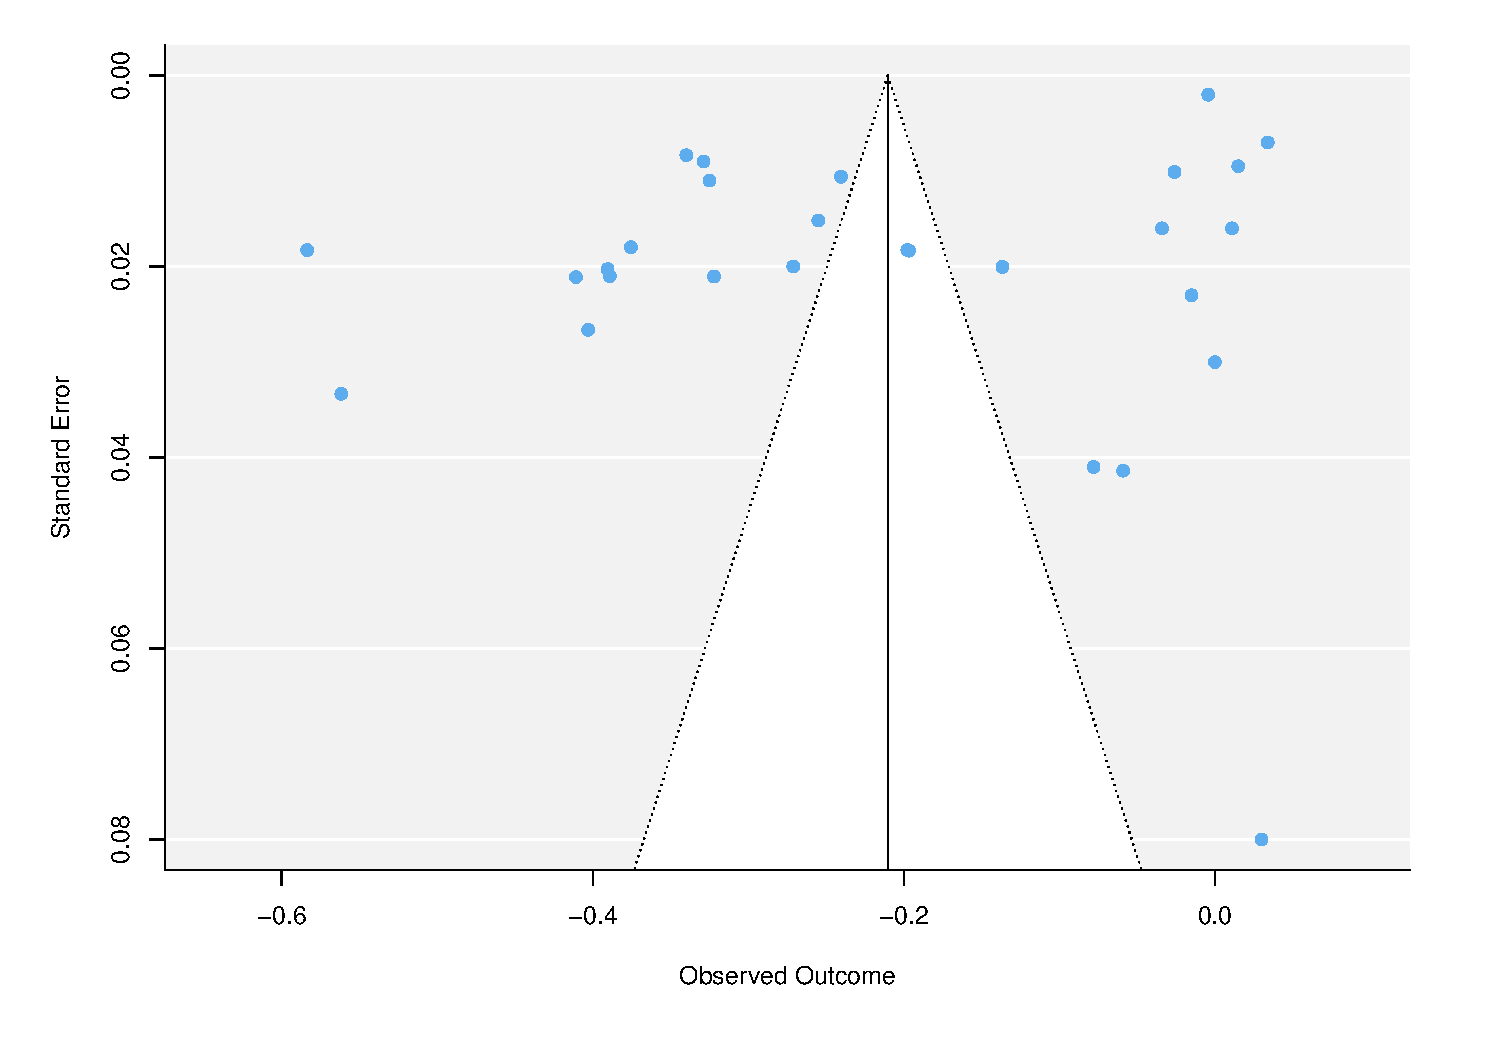
\includegraphics[scale = 0.45]{../figs/funnel_re_all.pdf}
\vspace{-0.2cm}
\caption{Funnel plot: All experiments}
\small
\vspace{-0.5cm}
\label{fig: funnel_all}
\end{figure}
\end{frame}

%%%%%%%%%%%%%%%%%%%%%%%%%%%%%%%%%%%

\begin{frame}[label=supplemental, noframenumbering]
\frametitle{Funnel plot asymmetry \hyperlink{pub_bias}{\beamerbutton{Back}}}

\begin{figure}[!hb]
\vspace*{-3mm}
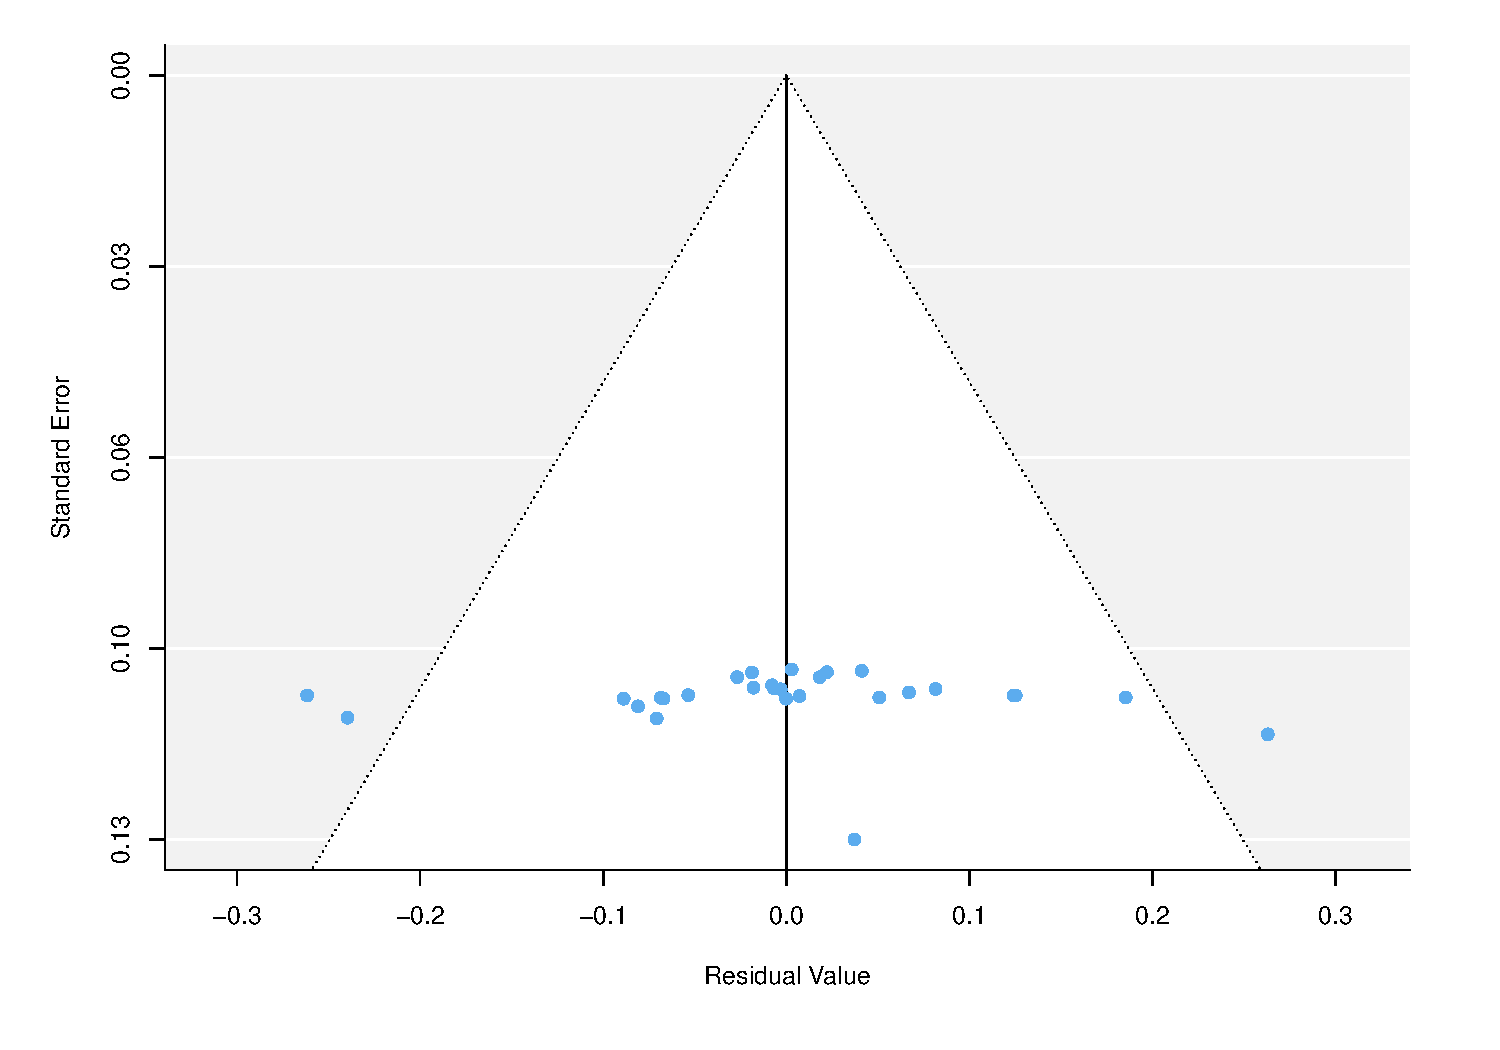
\includegraphics[scale = 0.45]{../figs/funnel_all_mod.pdf}
\vspace{-0.2cm}
\caption{Funnel plot: All experiments with field experiment moderator}
\small
\vspace{-0.5cm}
\label{fig: funnel_all}
\end{figure}
\end{frame}

%%%%%%%%%%%%%%%%%%%%%%%%%%%%%%%%%%%

\begin{frame}[label=supplemental, noframenumbering]
\frametitle{Funnel plot asymmetry \hyperlink{pub_bias}{\beamerbutton{Back}}}

\begin{figure}[!hb]
\vspace*{-3mm}
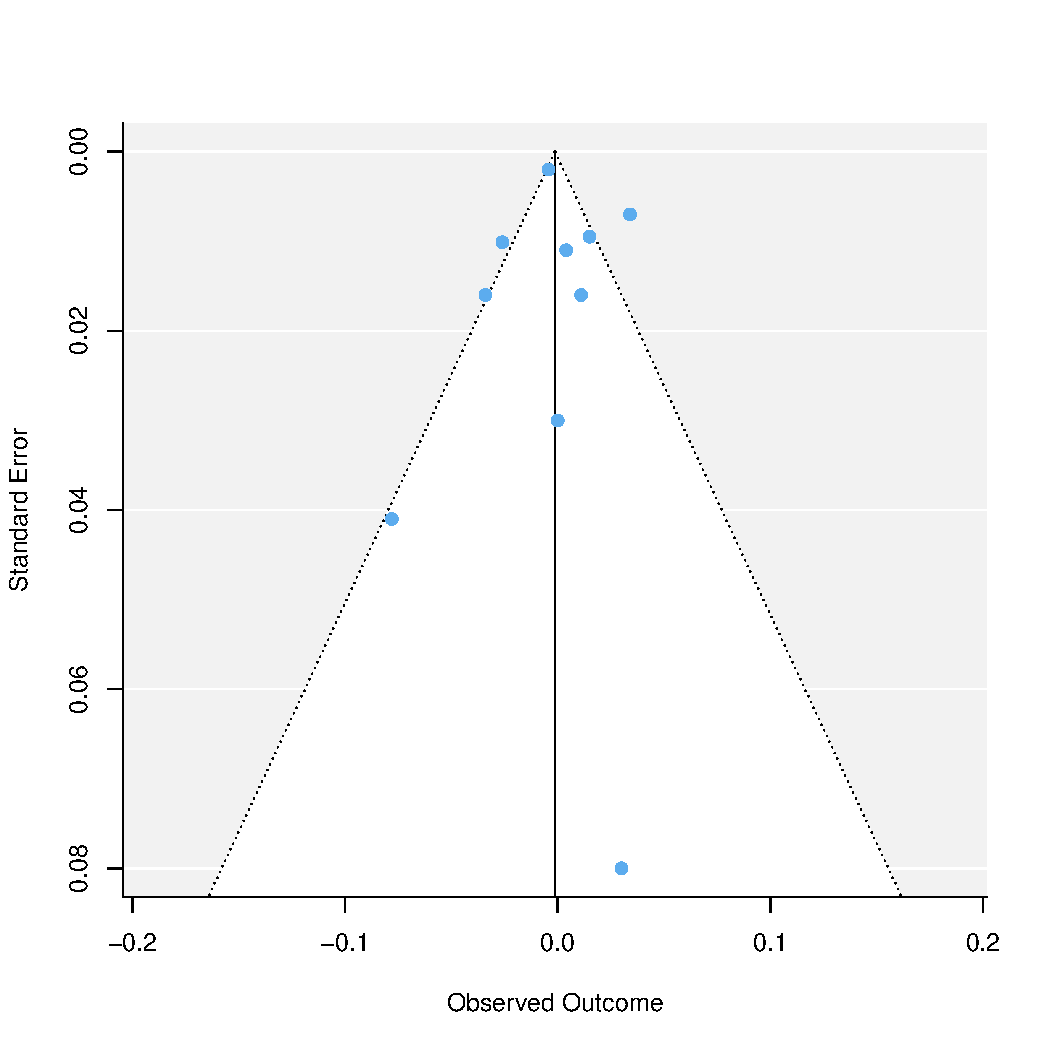
\includegraphics[scale = 0.45]{../figs/funnel_re_field.pdf}
\vspace{-0.2cm}
\caption{Funnel plot: Field experiments}
\small
\vspace{-0.5cm}
\label{fig: funnel_all}
\end{figure}
\end{frame}

%%%%%%%%%%%%%%%%%%%%%%%%%%%%%%%%%%%

\begin{frame}[label=p_ols_logit, noframenumbering]
\frametitle{Does p-value predict publication status? \hyperlink{pub_bias}{\beamerbutton{Back}}}

\footnotesize

% Table created by stargazer v.5.2.2 by Marek Hlavac, Harvard University. E-mail: hlavac at fas.harvard.edu
% Date and time: Wed, Jun 26, 2019 - 15:53:40
% Requires LaTeX packages: dcolumn 
\begin{table}[!htbp] \centering 
  \caption{Do p-values predict publication status?} 
  \label{p_publication} 
\begin{tabular}{@{\extracolsep{5pt}}lD{.}{.}{-2} D{.}{.}{-2} } 
\\[-1.8ex]\hline 
\hline \\[-1.8ex] 
 & \multicolumn{2}{c}{\textit{Dependent variable:}} \\ 
\cline{2-3} 
\\[-1.8ex] & \multicolumn{2}{c}{Published} \\ 
 & \multicolumn{1}{c}{OLS} & \multicolumn{1}{c}{Logit} \\ 
\hline \\[-1.8ex] 
 Reference: P less than 0.01 & 0.89^{***} & 2.08^{***} \\ 
  & (0.10) & (0.75) \\ 
  P less than 0.05 & -0.39 & -2.08^{*} \\ 
  & (0.23) & (1.25) \\ 
  P less than 0.1 & 0.11 & 14.49 \\ 
  & (0.42) & (2,399.54) \\ 
  P greater than 0.1 & -0.39^{*} & -2.08^{*} \\ 
  & (0.19) & (1.11) \\ 
 \hline \\[-1.8ex] 
Observations & \multicolumn{1}{c}{29} & \multicolumn{1}{c}{29} \\ 
\hline 
\hline \\[-1.8ex] 
\textit{Note:}  & \multicolumn{2}{r}{$^{*}$p$<$0.1; $^{**}$p$<$0.05; $^{***}$p$<$0.01} \\ 
\end{tabular} 
\end{table} 


\end{frame}

%%%%%%%%%%%%%%%%%%%%%%%%%%%%%%%%%%%

\begin{frame}[label=all_published, noframenumbering]
\frametitle{All experiments by publication status \hyperlink{pub_bias}{\beamerbutton{Back}}}

\begin{figure}[!htb]
\begin{centering}
\vspace{-0.2cm}
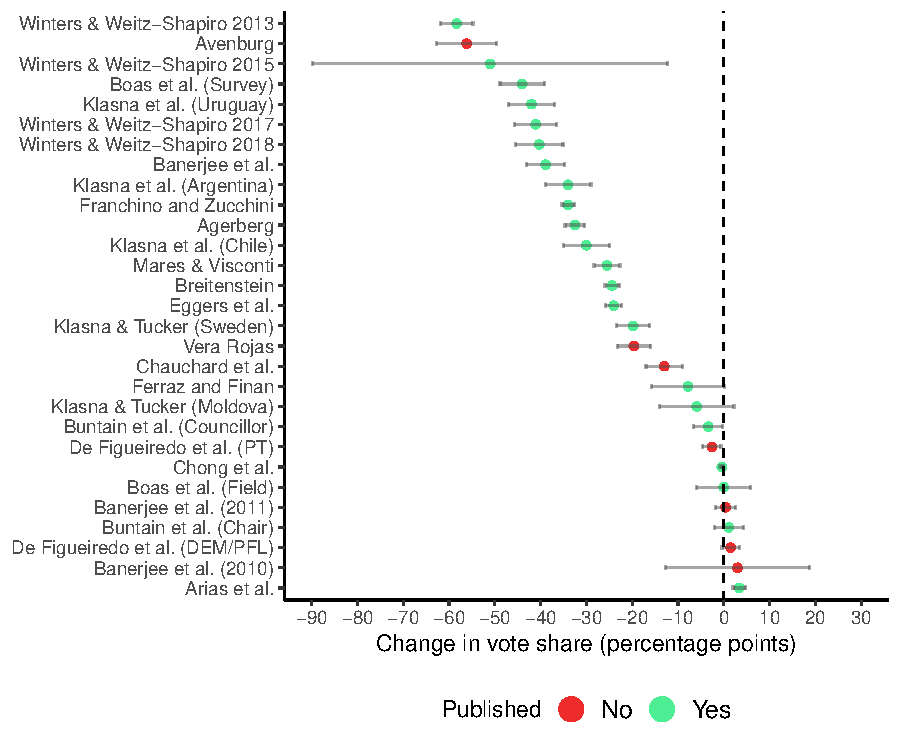
\includegraphics[scale=0.51]{../figs/published.pdf}
\caption{All experiments by publication status: Average treatment effect of corruption information on vote share and 95\% confidence intervals}.
\label{fig: funnel_re_survey}
\end{centering}
\end{figure}

\end{frame}

%%%%%%%%%%%%%%%%%%%%%%%%%%%%%%%%%%%

\begin{frame}[label=fz_conjoint1, noframenumbering]
\frametitle{Additional conjoint replications: \citet{franchino2015voting} \hyperlink{conjoint}{\beamerbutton{Back}}}

\begin{figure}[!htb]
\begin{centering}
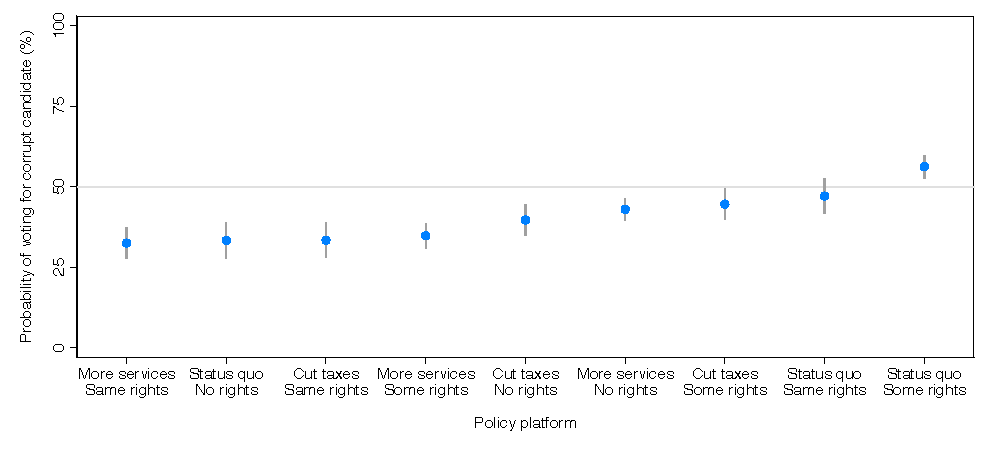
\includegraphics[scale=0.7]{../figs/fz_margins_right.pdf}
\caption{\citet{franchino2015voting} conjoint: can policy positions overcome corruption (conservative respondents)?}
\label{fig: funnel_re_survey}
\end{centering}
\end{figure}

\end{frame}

%%%%%%%%%%%%%%%%%%%%%%%%%%%%%%%%%%%

\begin{frame}[label=fz_conjoint2, noframenumbering]
\frametitle{Additional conjoint replications: \citet{franchino2015voting} \hyperlink{conjoint}{\beamerbutton{Back}}}

\begin{figure}[!htb]
\begin{centering}
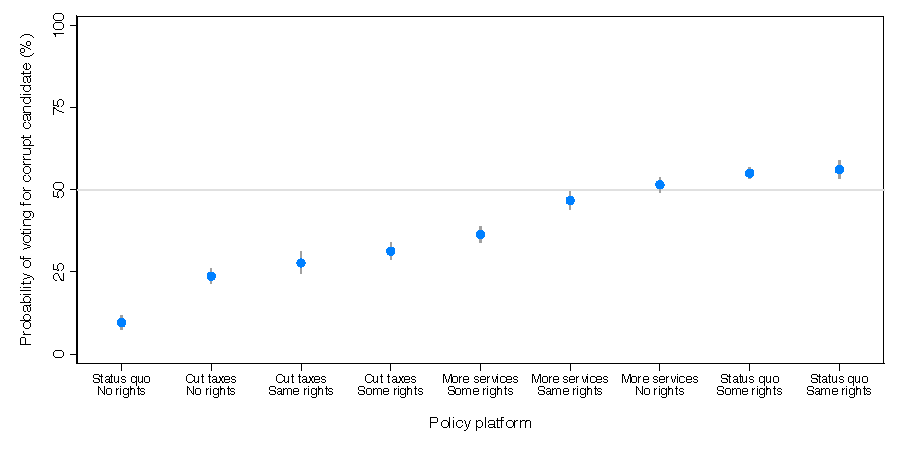
\includegraphics[scale=0.7]{../figs/fz_margins_left.pdf}
\caption{\citet{franchino2015voting} conjoint: can policy positions overcome corruption (liberal respondents)?}
\label{fig: funnel_re_survey}
\end{centering}
\end{figure}

\end{frame}

%%%%%%%%%%%%%%%%%%%%%%%%%%%%%%%%%%%

\bibliography{bibliography}
\end{document}